\subsection{Gleichspannungswandler}
	Das Ziel von Gleichspannungswandlern ist es m�glichst verlustarm Gleichspannung entweder hochzuwandeln oder runterzuwandeln. Diese Spannungswandler werden in 3 Kategorien geteilt.
	
	\subsubsection{Tiefsetzsteller(Buck-Converter)}
		Der Tiefsetzsteller funktioniert mithilfe von einem Schalttransistor (meist ein MOSFET) welches mit einem bestimmten Duty-Cycle(Tastgrad) ein- und ausgeschalten wird. Wenn der Schalter geschlossen ist, steigt der Strom durch die Induktivit�t langsam an und es flie�t kein Strom durch die Diode. Wenn der Schalter nun ge�ffnet sinkt der Strom der durch die Diode flie�t linear ab und der Strom flie�t nun durch
	
	\begin{figure}[H]
		\centering
		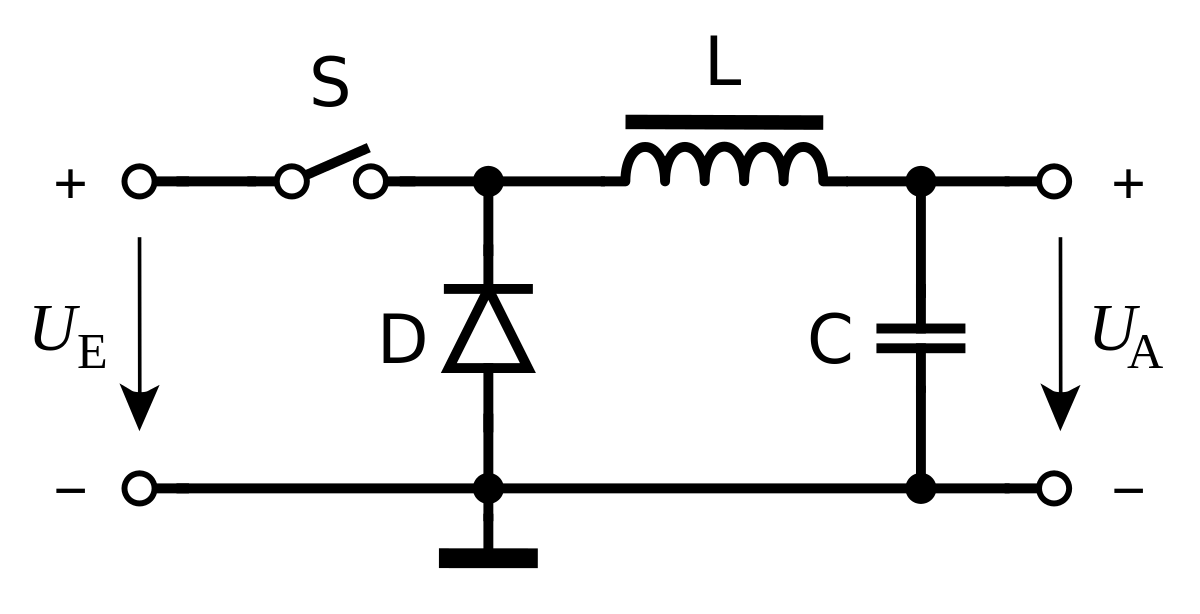
\includegraphics[scale=0.2]{./3_Stand_der_Technik/Abbildungen/Spannungswandler_1}
		\caption{Schaltbild eines Tiefsetzstellers\cite{wikipedia2024a}}
	\end{figure}
	
	\subsubsection{Hochsetzsteller(Boost-Converter)}
	
	\subsubsection{Hoch- und Tiefsetzsteller(Buck- and Boost-Converter)}